% Single-file LaTeX source: upload the fig_*.pdf (or .png) files to the same Overleaf project root.
\documentclass[11pt,a4paper]{article}
\usepackage[margin=2.4cm]{geometry}
\usepackage[T1]{fontenc}
\usepackage{lmodern}
\usepackage{microtype}
\usepackage{placeins}
\usepackage{needspace}
\usepackage{fancyhdr}
\usepackage{amsmath,amssymb}
\usepackage{booktabs,tabularx,float,graphicx}
\usepackage[font=small,labelfont=bf]{caption}
\usepackage[authoryear,round]{natbib}
\usepackage{xcolor}
\usepackage{listings}
\usepackage[hidelinks]{hyperref}
\usepackage{enumitem}
\usepackage{adjustbox}
\graphicspath{{./}{figures/}{../figures/}}
\setlist{itemsep=2pt,topsep=3pt}
\setlength{\parskip}{4pt}
\setlength{\parindent}{0pt}
\pagestyle{fancy}\fancyhf{}
\fancyhead[L]{\small\itshape Realized volatility forecasting, Indian equities}
\fancyhead[R]{\small\itshape Guntur \& Panchal (2026)}
\fancyfoot[C]{\small\thepage}
\renewcommand{\headrulewidth}{0.3pt}
\setlength{\headheight}{14pt}
\setlength{\floatsep}{10pt plus 2pt}
\setlength{\textfloatsep}{12pt plus 2pt}
\setlength{\intextsep}{10pt plus 2pt}
\renewcommand{\floatpagefraction}{0.75}
\let\oldsection\section
\renewcommand{\section}{\FloatBarrier\needspace{6\baselineskip}\oldsection}
\definecolor{codebg}{HTML}{F6F6F4}
\lstset{language=Python,basicstyle=\ttfamily\scriptsize,backgroundcolor=\color{codebg},
  frame=single,rulecolor=\color{gray!40},breaklines=true,columns=fullflexible,
  keywordstyle=\color{blue!60!black},commentstyle=\color{gray},stringstyle=\color{teal!70!black},
  showstringspaces=false,aboveskip=4pt,belowskip=4pt}

\begin{document}
\begin{titlepage}
\centering
\vspace*{2.2cm}
{\LARGE\bfseries Forecasting Realized Volatility of Indian Equities\par}
\vspace{6pt}
{\Large HAR-RV, EGARCH and LSTM Models across Liquidity Groups\par}
\vspace{14pt}
{\large 95 NIFTY 100 stocks $\cdot$ 5-minute NSE data $\cdot$ January 2016 -- April 2026\par}
\vspace{1.6cm}
{\large Partha Guntur \quad and \quad Rajvi Panchal\par}
\vspace{6pt}
M.Sc. Quantitative Finance, Ahmedabad University\par
AI Lab Project, Category 2: Research-Based\par
\vspace{10pt}
November 2026\par
\vspace{1.4cm}
\begin{minipage}{0.9\textwidth}\small\setlength{\parskip}{4pt}
{\centering\textbf{Abstract}\par}\vspace{6pt}
\noindent We forecast next-day realized volatility for 95 NIFTY~100 stocks using 5-minute NSE data
(2016--2026) and ask whether deep learning beats the HAR benchmark, and whether the answer depends
on liquidity. On 29,774 out-of-sample stock-days (January 2025 -- April 2026), an LSTM fed with HAR
inputs (HAR-RV-LSTM) is the most accurate model: its QLIKE loss is 15.4\% below HAR-RV and 1.6\% below
log-HAR, both statistically significant. It beats HAR-RV on all 95 stocks and log-HAR on 70\% of them.
Its edge over log-HAR rises as liquidity falls, from 0.3\% (not significant) for the most liquid third
to 3.0\% for the least liquid third. An LSTM built on EGARCH features is the weakest model, and EGARCH
features add nothing to HAR-RV-LSTM. The gains come from calm and normal days. Correcting data errors,
the liquidity measure and look-ahead in the EGARCH features made the benchmark much stronger and the
neural models' advantage smaller than in our first version.

\medskip
\noindent\textbf{Keywords:} realized volatility, HAR, LSTM, EGARCH, liquidity, NSE, forecast evaluation\\
\textbf{JEL codes:} C45, C53, C58, G17

\end{minipage}
\vfill
\end{titlepage}

\tableofcontents
\clearpage

\section{Introduction}

Volatility is the main input to option pricing, margin setting, Value-at-Risk and position sizing,
but it cannot be observed directly. With intraday data it can be measured: the sum of squared 5-minute
returns gives a day's realized variance (RV), and forecasting RV has become the standard way to forecast
volatility \citep{andersen2003}. The benchmark is the HAR model of \citet{corsi2009}, a linear
regression of tomorrow's RV on its daily, weekly and monthly averages. It is simple and hard to beat.

Neural networks, in particular LSTMs, are often reported to beat HAR, but the gains are uneven and
the evidence comes mostly from liquid US stocks \citep{bucci2020,rahimikia2020,christensen2023}.
In less liquid stocks RV is a noisier measurement, which points two ways. A flexible model may find more
structure to exploit there (H1), or it may mostly fit noise and gain only in liquid stocks (H2).
Indian large caps span a wide range of liquidity --- average daily turnover in our sample runs from
about Rs~9 crore to Rs~1,360 crore --- so they are a natural place to test this.

\needspace{8\baselineskip}
We ask four questions:
\begin{enumerate}
\item Does an LSTM fed with HAR inputs (HAR-RV-LSTM) forecast next-day RV better than HAR-RV and log-HAR?
\item Does an LSTM fed with EGARCH features from daily returns do as well, and do EGARCH features add
anything to the HAR inputs?
\item Does the gain depend on the stock's liquidity (H1 against H2)?
\item Does it depend on market conditions, and is it stable over time and across training runs?
\end{enumerate}

\textbf{Main findings.} HAR-RV-LSTM is the most accurate model on every loss. Against classic HAR-RV it
reduces QLIKE by 15.4\%; against log-HAR, the fairer benchmark, by 1.6\%. Both differences are
significant, every training seed beats log-HAR, and the gain rises from 0.3\% in the most liquid stocks to
3.0\% in the least liquid, which supports H1. EGARCH-LSTM is worse than plain HAR-RV, and EGARCH features
add nothing to HAR-RV-LSTM. The gain is concentrated on calm and normal days.

\textbf{Contributions.} (i) A cleaned, reproducible 5-minute panel for 95 NSE stocks with documented
rules for pre-listing rows, bad prints and corporate actions. (ii) A liquidity-conditioned comparison
of econometric and deep-learning volatility models on an emerging market, with liquidity groups formed
only from training-period data. (iii) An honest account of how three implementation errors in our
first version --- uncleaned RV, a mis-scaled liquidity measure and EGARCH look-ahead --- had inflated
the apparent advantage of the neural models (Section~\ref{sec:versions}).

\section{Literature Review}

\textbf{Realized volatility.} Summing squared intraday returns gives realized variance (RV), a
model-free estimate of the day's integrated variance \citep{andersen2003}. Five-minute sampling is
hard to beat across asset classes \citep{liu2015}, and simple models of RV forecast better than
GARCH models fitted to daily returns \citep{andersen2003}.

\textbf{HAR-RV.} \citet{corsi2009} regresses tomorrow's RV on its daily, weekly and monthly
averages. Four parameters reproduce the long memory of volatility, and the model is still the
standard benchmark. Estimating it in logs reduces the weight of a few extreme days on the
coefficients.

\textbf{EGARCH and hybrids.} EGARCH \citep{nelson1991} models log variance from daily returns and
allows bad news to raise volatility more than good news. \citet{kim2018} feed GARCH-family outputs
into an LSTM \citep{hochreiter1997} for the KOSPI 200 and report gains over both parts.

\textbf{Machine learning against HAR.} \citet{bucci2020} finds recurrent networks beat HAR models
for US equity RV. Large DJIA studies are more sceptical: \citet{rahimikia2020} find gains mainly in
calm periods, and \citet{christensen2023} find they depend on covariates and the evaluation window.
Pooling many stocks in one network helps \citep{zhang2024}. Almost all of this evidence is for
liquid US stocks; whether the gain depends on liquidity, and whether it holds in an emerging market,
is largely untested.

\textbf{Evaluation.} RV is itself an estimate, so the loss must rank forecasts correctly under a noisy
proxy; MSE and QLIKE do, and QLIKE is less sensitive to extreme days \citep{patton2011}. Forecasts are
compared with the Diebold--Mariano test \citep{diebold1995}, with Newey--West standard errors
\citep{neweywest1987}.

\section{Data}

\subsection{Source and cleaning}

The data are 5-minute bars (open, high, low, close, volume) for 100 current NIFTY~100 stocks on the
NSE, February 2015 to 9 April 2026 (18.8 million bars). The regular session runs 09:15--15:30 IST, so
a full day has 75 bars. Prices are mostly adjusted for corporate actions, but the files contain
pre-listing quotes, zero prices, special sessions and isolated bad prints. Table~\ref{tab:cleaning}
lists the rules; all are set in one configuration file.

\begin{table}[htbp]
\centering
\caption{Data cleaning rules and their effect}
\label{tab:cleaning}
\small
\begin{adjustbox}{max width=\textwidth}
\begin{tabular}{lcr}
\toprule
Rule & Action & Count \\
\midrule
Raw 5-minute bars, 100 stocks & -- & 18,798,744 \\
Regular session 09:15--15:30, from Nov 2015, after listing date & Keep & 17,660,206 \\
Zero-volume bars (stale quote, price set to missing) & Drop price & 41,063 \\
Isolated spikes ($>$5\% move undone by next bar) & Drop price & 24 \\
Days with fewer than 60 traded bars & Drop day & 1,455 \\
Days with RV $=0$ (stock frozen at price band) & Drop day & 188 \\
Overnight gaps $>35\%$ (split/bonus) in EGARCH returns & Set to 0 & 2 \\
Stock-days in the clean panel & -- & 234,226 \\
\bottomrule
\end{tabular}
\end{adjustbox}
\par\smallskip\parbox{0.95\textwidth}{\footnotesize\itshape Pre-listing rows removed for IRFC, SBILIFE, HDFCLIFE and MAZDOCK. RV never uses overnight returns.}
\end{table}


The most volatile stock-days left after cleaning are real events: the Adani sell-off of 1--3 February
2023 and the COVID-19 crash of March 2020 (Annex Table~\ref{tab:topdays}).

\subsection{Realized variance and returns}

Let $r_{i,t,j}$ be the $j$-th 5-minute log return of stock $i$ on day $t$, with the first return measured
from the day's first traded open. Realized variance is
\begin{equation}
RV_{i,t}=\sum_{j=1}^{M_{i,t}} r_{i,t,j}^{2}, \qquad M_{i,t}\le 75 .
\end{equation}
RV covers the trading session only; the overnight gap is excluded, which keeps unadjusted splits,
bonus issues and demergers out of the target. Annualized volatility is $\sqrt{252\,RV}$. Daily
close-to-close returns for EGARCH add the overnight return, set to zero on the two days where it
exceeded 35\% in absolute value (a corporate action, not a price move).

\subsection{Sample split and universe}

Each observation is assigned to a period by the date of the \emph{target} (day $t+1$): training
2016--2022, validation 2023--2024 (early stopping only), and test 1 January 2025 -- 9 April 2026,
which was not used for any choice. The universe is the 95 stocks with at least 250 training days;
five recent listings (Hyundai, Jio Financial, Tata Capital, TMCV, ENRIN) are excluded.

\subsection{Liquidity groups}

Liquidity is measured with the 5-minute Amihud ratio \citep{amihud2002},
\begin{equation}
ILLIQ_i=\frac{1}{N_i}\sum_{k}\frac{|r_{i,k}|}{\text{Rupee volume}_{i,k}},
\end{equation}
averaged over all traded 5-minute bars in the \emph{training} years only, so group membership uses
no information from the evaluation period. A low ILLIQ means trades move the price little. Stocks are
split into terciles: High (32 stocks), Medium (31) and Low liquidity (32). The ranking agrees with
traded value (Spearman $-0.91$): Reliance, SBI, Infosys and ICICI Bank are the most liquid; CG Power,
Solar Industries and Trent the least (Figure~\ref{fig:liq}).

\begin{figure}[htbp]
\centering
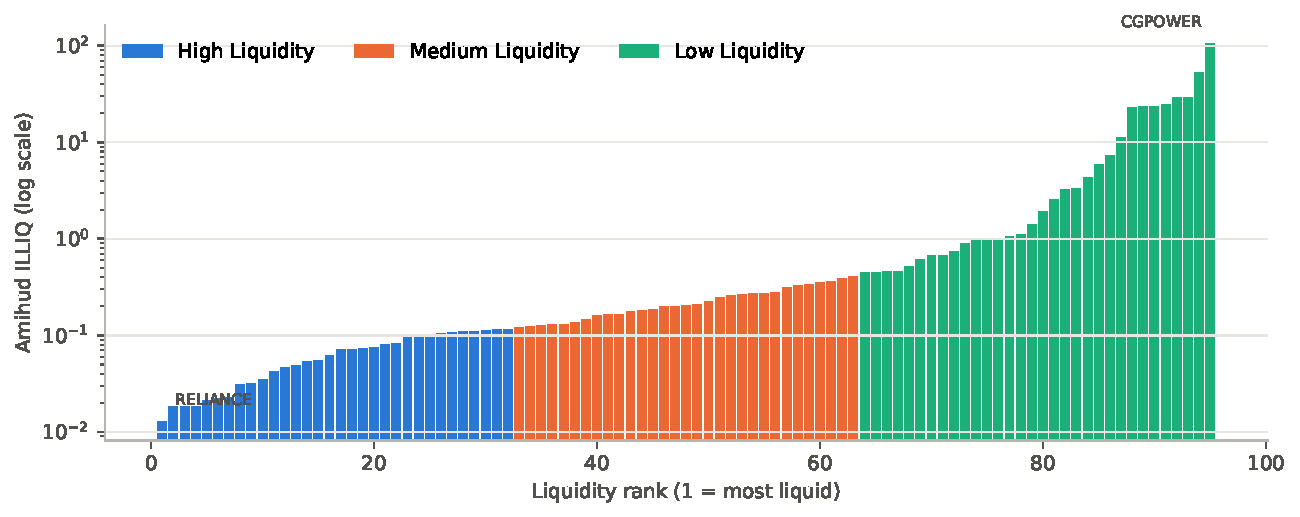
\includegraphics[width=\textwidth]{fig_liquidity_ranking}
\caption{Amihud illiquidity of the 95 stocks in the training years (log scale), coloured by tercile.}
\label{fig:liq}
\end{figure}

\begin{table}[htbp]
\centering
\caption{The three liquidity groups, 2016--2026}
\label{tab:desc}
\small
\begin{adjustbox}{max width=\textwidth}
\begin{tabular}{lrrrrrrr}
\toprule
Liquidity & Stocks & Stock-days & Turnover (Rs cr/day) & Mean vol (\%) & Median vol (\%) & 99th pct vol (\%) & AR(1) log RV \\
\midrule
High & 32 & 80,742 & 533 & 25.1 & 22.0 & 75.6 & 0.70 \\
Medium & 31 & 78,064 & 193 & 28.5 & 25.3 & 81.4 & 0.65 \\
Low & 32 & 73,900 & 142 & 33.1 & 28.4 & 103.8 & 0.65 \\
\bottomrule
\end{tabular}
\end{adjustbox}
\par\smallskip\parbox{0.95\textwidth}{\footnotesize\itshape Vol = annualized intraday realized volatility $\sqrt{252\,RV}$. Turnover measured in the training years.}
\end{table}


Less liquid stocks are more volatile and their volatility is less persistent
(Table~\ref{tab:desc}): the first-order autocorrelation of log RV is 0.70 for the most liquid third and
0.65 for the other two.

\begin{figure}[htbp]
\centering
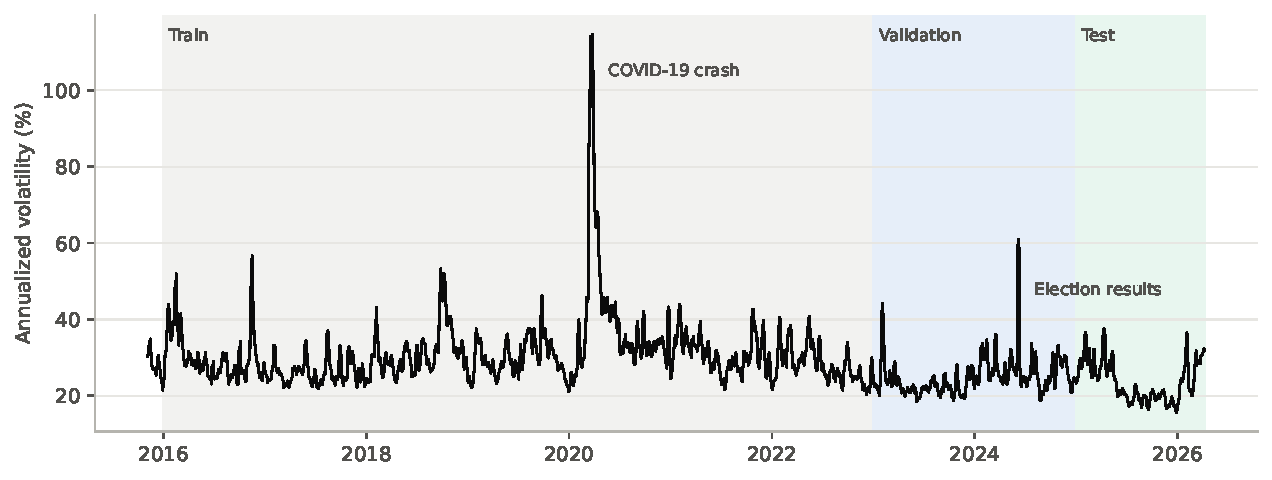
\includegraphics[width=\textwidth]{fig_rv_timeline}
\caption{Average annualized intraday volatility across the 95 stocks (5-day average) with the three
sample periods.}
\label{fig:timeline}
\end{figure}

The test period is calmer than training on average (Figure~\ref{fig:timeline}), but it includes the
tariff shock of April 2025 and the rise in volatility in early 2026.

\section{Methodology}

\subsection{Econometric benchmarks}

\textbf{HAR-RV} \citep{corsi2009}, estimated by OLS separately for each stock:
\begin{equation}
RV_{t+1}=\beta_0+\beta_D RV_t+\beta_W RV^{(5)}_t+\beta_M RV^{(22)}_t+\varepsilon_{t+1},
\end{equation}
where $RV^{(5)}_t$ and $RV^{(22)}_t$ are 5- and 22-day averages. \textbf{log-HAR} is the same
regression in logs, with forecast $\exp(\hat y+s^2/2)$ to correct for the log-normal bias. Validation
forecasts use coefficients from 2016--2022; test forecasts re-estimate on 2016--2024.

\textbf{EGARCH(1,1)-t} \citep{nelson1991} for daily returns,
\begin{equation}
\log\sigma_t^2=\omega+\beta\log\sigma_{t-1}^2+\alpha\left(|z_{t-1}|-E|z_{t-1}|\right)+\gamma z_{t-1},
\end{equation}
with Student-$t$ errors. Parameters are estimated on 2016--2022 only and then held fixed while the
model runs forward, so every feature on day $t$ uses returns up to $t$ and parameters that never saw
the evaluation years. The leverage term $\gamma$ is negative for 92\% of stocks (mean $-0.042$),
and persistence $\beta$ averages 0.92 (Annex Table~\ref{tab:egarch}).

\subsection{LSTM models}

All three networks share one architecture and training rule; only the inputs differ
(Table~\ref{tab:lstm}). A single network is trained on all 95 stocks. Each input is the last 22
trading days of features for one stock; a learned 8-dimensional stock embedding lets the network
adjust to each stock's volatility level. The output is $\exp(z+c)$, which is always positive, with
$c$ the mean training log RV. Inputs are logged where relevant and standardized with training-period
means. The loss is QLIKE. Each model is trained with three random seeds and the reported forecast is
the average of the three.

\begin{table}[htbp]
\centering
\caption{LSTM inputs and training settings}
\label{tab:lstm}
\small
\begin{tabularx}{\textwidth}{lX}
\toprule
Model & Inputs for each of the last 22 days \\
\midrule
HAR-RV-LSTM & $\log RV_t$, $\log RV^{(5)}_t$, $\log RV^{(22)}_t$ \\
EGARCH-LSTM & $\log \hat\sigma_t$ (EGARCH volatility), $z_t$ (EGARCH standardized shock) \\
HAR-EGARCH-LSTM & all five (ablation) \\
\midrule
Network & 2-layer LSTM (64 units, dropout 0.2) $\rightarrow$ [last hidden state, stock embedding (8)] $\rightarrow$ 64 $\rightarrow$ 32 $\rightarrow$ 1 \\
Training & Adam, learning rate $10^{-3}$ halved on plateau, weight decay $10^{-4}$, batch 256, gradient clipping 1.0, early stopping on validation QLIKE (patience 8, max 60 epochs) \\
Seeds & 11, 22, 33; forecast = average of the three networks \\
\bottomrule
\end{tabularx}
\end{table}

HAR-RV-LSTM sees exactly the information HAR uses, so any gain comes from the non-linear,
sequence-based and pooled form of the model rather than from new data. EGARCH-LSTM sees only
daily-return information. The networks are trained once and not re-trained on validation data,
whereas the HAR benchmarks are re-estimated on 2016--2024 before the test; this favours HAR.

\subsection{Evaluation}

For forecast $h$ and realized variance $RV$:
\begin{equation}
\text{MSE}=(RV-h)^2,\qquad \text{MAE}=|RV-h|,\qquad \text{QLIKE}=\frac{RV}{h}-\log\frac{RV}{h}-1 .
\end{equation}
QLIKE is the main loss \citep{patton2011}. Losses are computed on the same 29,774 test stock-days for
every model. Significance uses a panel Diebold--Mariano test \citep{diebold1995}: the loss
difference is averaged across stocks each day, and the mean of that daily series is tested with
Newey--West (5 lags) standard errors; $p$-values are Holm-adjusted within each loss. A moving-block
bootstrap (5-day blocks, 2,000 draws) gives a second confidence interval. Calibration is checked with
Mincer--Zarnowitz regressions in logs, with standard errors clustered by date.

\section{Results: Overall Accuracy}

\begin{table}[htbp]
\centering
\caption{Forecast accuracy, validation and test periods}
\label{tab:overall}
\small
\begin{adjustbox}{max width=\textwidth}
\begin{tabular}{lrrrrrr}
\toprule
Model & Valid QLIKE & Test QLIKE & Test MAE ($\times10^{4}$) & Test MSE ($\times10^{8}$) & vs HAR-RV (\%) & vs log-HAR (\%) \\
\midrule
HAR-RV & 0.2606 & 0.2286 & 1.656 & 9.303 & -- & +16.3 \\
log-HAR & 0.2298 & 0.1965 & 1.432 & 8.597 & $-$14.0 & -- \\
HAR-RV-LSTM & 0.2258 & \textbf{0.1935} & \textbf{1.401} & \textbf{8.543} & $-$15.4 & $-$1.6 \\
EGARCH-LSTM & 0.2703 & 0.2709 & 2.034 & 11.856 & +18.5 & +37.8 \\
\midrule
HAR-EGARCH-LSTM & 0.2184 & 0.1931 & 1.444 & 8.703 & $-$15.5 & $-$1.7 \\
\bottomrule
\end{tabular}
\end{adjustbox}
\par\smallskip\parbox{0.95\textwidth}{\footnotesize\itshape Test: 29,774 stock-days, 95 stocks, 1 Jan 2025 -- 9 Apr 2026; validation: 46,599 stock-days, 2023--2024. Last two columns: change in test QLIKE (negative = better). Bold = lowest test loss among the four main models. HAR-EGARCH-LSTM is an ablation.}
\end{table}


\textbf{Ranking.} HAR-RV-LSTM has the lowest test loss on all three measures (Table~\ref{tab:overall},
Figure~\ref{fig:losses}). Its QLIKE of 0.1935 is 15.4\% below HAR-RV and 1.6\% below log-HAR.
EGARCH-LSTM is the weakest model, 18.5\% worse than HAR-RV. The validation ranking is the same.

\textbf{Where the gain over HAR-RV comes from.} log-HAR alone removes 14.0 of the 15.4 points.
Level HAR-RV is pulled up by a few extreme training days and over-forecasts by 21\% on average
(Table~\ref{tab:mz}). The network's own contribution, beyond working in logs, is the remaining 1.6\%.

\begin{figure}[htbp]
\centering
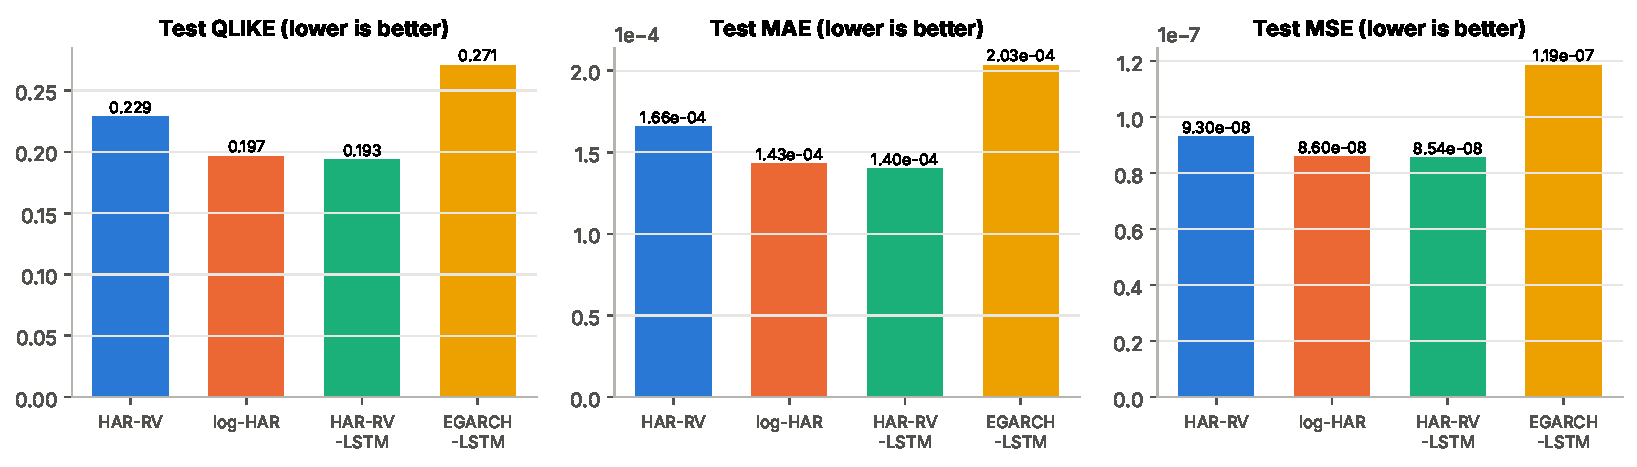
\includegraphics[width=\textwidth]{fig_test_losses}
\caption{Test-period losses of the four main models (lower is better).}
\label{fig:losses}
\end{figure}

\textbf{Significance.} All differences with HAR-RV are significant (Table~\ref{tab:dm}). HAR-RV-LSTM
against log-HAR: $t=2.80$, Holm $p=0.010$, and the bootstrap interval [0.0011, 0.0054] excludes zero.
On MAE the gain is also significant ($t=4.22$); on MSE it is not ($p=0.26$), because MSE is driven by a
handful of extreme days. Adding EGARCH features to HAR-RV-LSTM changes nothing ($t=0.24$, $p=0.81$).

\begin{table}[htbp]
\centering
\caption{Diebold--Mariano tests on the test period (A vs B)}
\label{tab:dm}
\small
\begin{adjustbox}{max width=\textwidth}
\begin{tabular}{lrrrcrr}
\toprule
Comparison & QLIKE diff (A$-$B) & $t$ & Holm $p$ & 95\% block-bootstrap CI & MAE $t$ & MAE Holm $p$ \\
\midrule
HAR-RV vs log-HAR & 0.0320 & 6.54 & $<$0.001 & [0.0235, 0.0417] & 11.02 & $<$0.001 \\
HAR-RV vs HAR-RV-LSTM & 0.0351 & 6.18 & $<$0.001 & [0.0250, 0.0465] & 10.11 & $<$0.001 \\
log-HAR vs HAR-RV-LSTM & 0.0031 & 2.80 & 0.010 & [0.0011, 0.0054] & 4.22 & $<$0.001 \\
HAR-RV vs EGARCH-LSTM & $-$0.0425 & $-$12.73 & $<$0.001 & [$-$0.0483, $-$0.0359] & $-$9.90 & $<$0.001 \\
log-HAR vs EGARCH-LSTM & $-$0.0745 & $-$10.39 & $<$0.001 & [$-$0.0885, $-$0.0611] & $-$14.90 & $<$0.001 \\
EGARCH-LSTM vs HAR-RV-LSTM & 0.0776 & 9.89 & $<$0.001 & [0.0631, 0.0929] & 14.92 & $<$0.001 \\
HAR-RV-LSTM vs HAR-EGARCH-LSTM & 0.0003 & 0.24 & 0.810 & [$-$0.0016, 0.0027] & $-$5.42 & $<$0.001 \\
\bottomrule
\end{tabular}
\end{adjustbox}
\par\smallskip\parbox{0.95\textwidth}{\footnotesize\itshape Positive difference / $t$ = model B has lower loss. Loss differences averaged across stocks per day (314 days), Newey--West (5 lags) standard errors; Holm adjustment over the seven comparisons per loss. Bootstrap: 5-day blocks, 2,000 draws.}
\end{table}


\textbf{Stability.} The gain builds steadily through the test period rather than coming from a few days
(Figure~\ref{fig:cum}): against log-HAR it is flat until June 2025 and rises after. Each of the three
seeds beats log-HAR on its own (test QLIKE 0.1926--0.1959 against 0.1965; Annex Table~\ref{tab:seeds}).
By stock, HAR-RV-LSTM beats HAR-RV on all 95 stocks and log-HAR on 67 of 95 (70\%).

\begin{figure}[htbp]
\centering
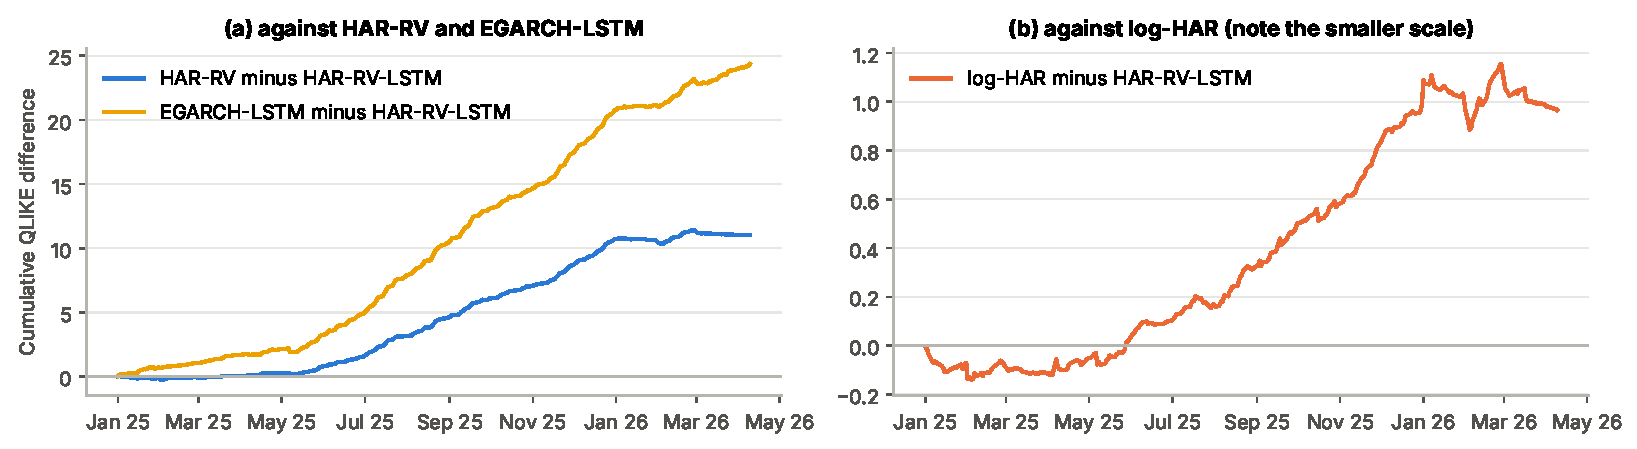
\includegraphics[width=\textwidth]{fig_cumulative_qlike}
\caption{Cumulative daily QLIKE difference against HAR-RV-LSTM over the test period. A rising line means
HAR-RV-LSTM is ahead.}
\label{fig:cum}
\end{figure}

\begin{figure}[htbp]
\centering
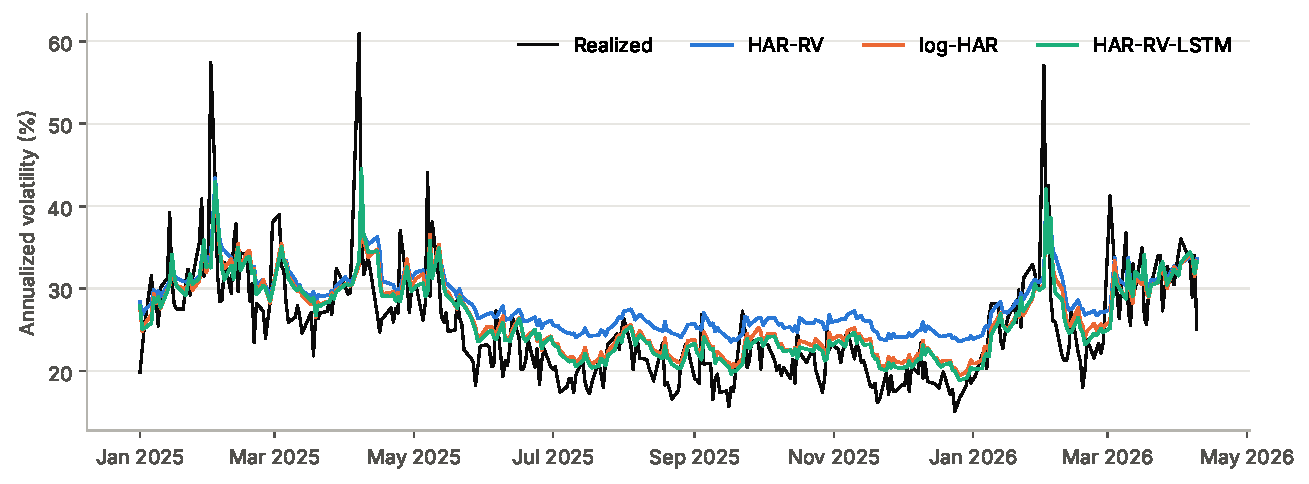
\includegraphics[width=\textwidth]{fig_forecast_vs_actual}
\caption{Average realized volatility across the 95 stocks and the average forecasts (annualized).}
\label{fig:fva}
\end{figure}

\textbf{Calibration.} HAR-RV sits visibly above realized volatility in the calm second half of 2025
(Figure~\ref{fig:fva}). In Mincer--Zarnowitz regressions HAR-RV-LSTM explains the most variation
($R^2=0.470$ against 0.462 for log-HAR) and has the smallest average bias (6\%).

\begin{table}[htbp]
\centering
\caption{Mincer--Zarnowitz regressions, test period: $\log RV_{t+1}=\alpha+\beta\log\hat h_{t+1}$}
\label{tab:mz}
\small
\begin{adjustbox}{max width=\textwidth}
\begin{tabular}{lrrrrr}
\toprule
Model & $\alpha$ & $\beta$ & s.e.($\beta$) & $R^2$ & Mean forecast / mean RV \\
\midrule
HAR-RV & $-$0.815 & 0.948 & 0.017 & 0.402 & 1.210 \\
log-HAR & $-$0.931 & 0.918 & 0.017 & 0.462 & 1.080 \\
HAR-RV-LSTM & $-$0.775 & 0.934 & 0.018 & 0.470 & 1.059 \\
EGARCH-LSTM & $-$2.193 & 0.790 & 0.014 & 0.348 & 1.395 \\
\bottomrule
\end{tabular}
\end{adjustbox}
\par\smallskip\parbox{0.95\textwidth}{\footnotesize\itshape A well-calibrated forecast has $\beta\approx1$. Standard errors clustered by date.}
\end{table}


\section{Results: Liquidity}

\begin{table}[htbp]
\centering
\caption{Test QLIKE by liquidity group}
\label{tab:liquidity}
\small
\begin{adjustbox}{max width=\textwidth}
\begin{tabular}{lrrrrrrrr}
\toprule
Liquidity & Obs & HAR-RV & log-HAR & HAR-RV-LSTM & EGARCH-LSTM & Gain vs HAR (\%) & Gain vs log-HAR (\%) & DM $t$ \\
\midrule
High & 10,026 & 0.2260 & 0.1920 & \textbf{0.1915} & 0.2477 & 15.3 & 0.3 & 0.38 \\
Medium & 9,716 & 0.2192 & 0.1925 & \textbf{0.1898} & 0.2556 & 13.4 & 1.4 & 2.43 \\
Low & 10,032 & 0.2403 & 0.2050 & \textbf{0.1989} & 0.3087 & 17.2 & 3.0 & 3.96 \\
\bottomrule
\end{tabular}
\end{adjustbox}
\par\smallskip\parbox{0.95\textwidth}{\footnotesize\itshape Gain = percentage reduction in QLIKE of HAR-RV-LSTM. DM $t$: HAR-RV-LSTM against log-HAR within the group (positive = LSTM better). Bold = best model in the group.}
\end{table}


HAR-RV-LSTM is the best model in every liquidity group (Table~\ref{tab:liquidity},
Figure~\ref{fig:liqq}). Its gain over log-HAR rises as liquidity falls: 0.3\% in the most liquid third
(not significant, $t=0.38$), 1.4\% in the middle third ($t=2.43$) and 3.0\% in the least liquid third
($t=3.96$). Across stocks the gain is positively correlated with the illiquidity rank (Spearman 0.29;
Figure~\ref{fig:perstock}). This supports H1: the network helps most where RV is noisiest and a linear
model fits worst. For the most liquid stocks, log-HAR is already as good.

EGARCH-LSTM falls further behind as liquidity falls (QLIKE 0.248 to 0.309): daily returns describe the
volatility of thinly traded stocks particularly poorly.

\begin{figure}[htbp]
\centering
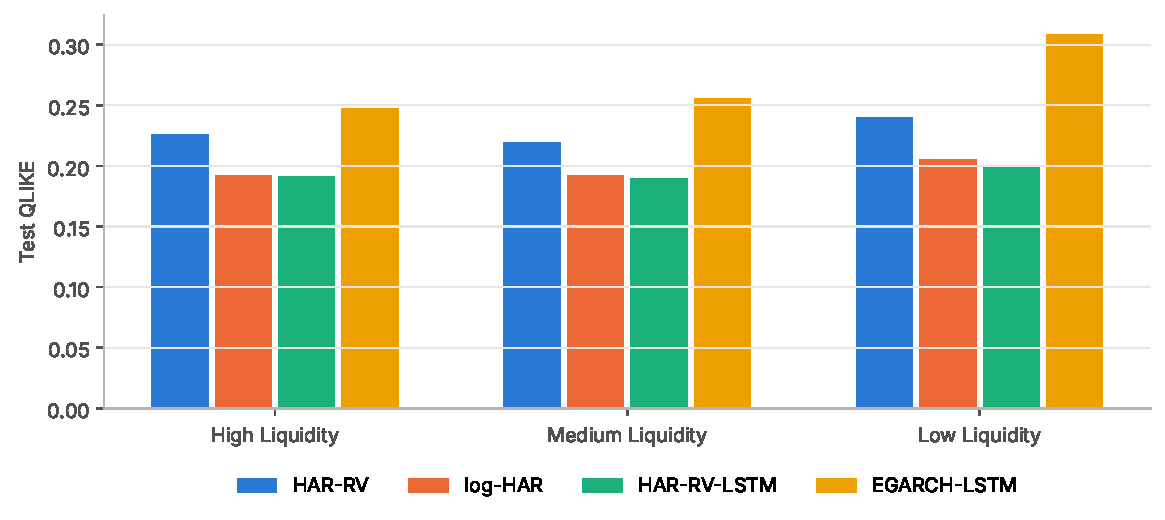
\includegraphics[width=0.85\textwidth]{fig_liquidity_qlike}
\caption{Test QLIKE by liquidity group.}
\label{fig:liqq}
\end{figure}

\begin{figure}[htbp]
\centering
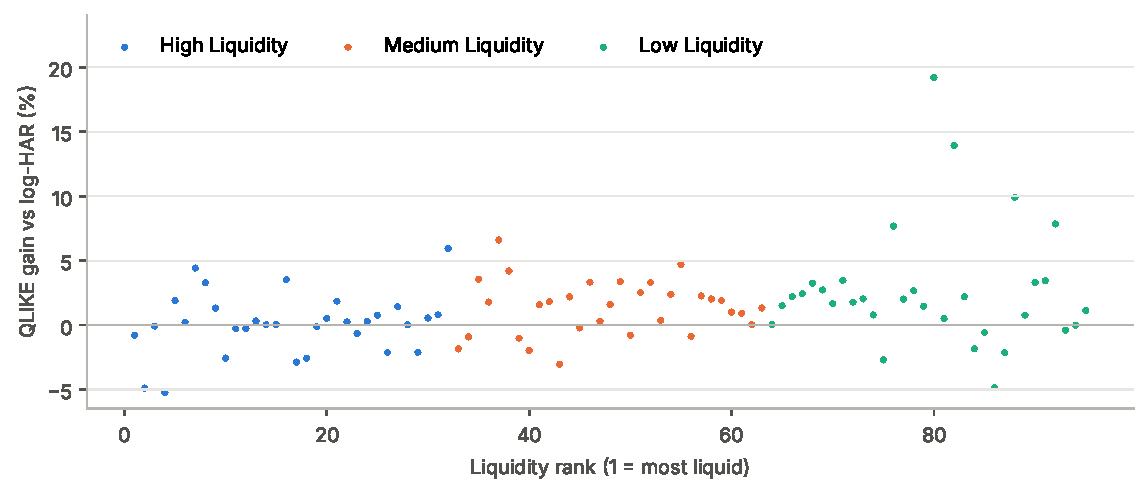
\includegraphics[width=0.85\textwidth]{fig_per_stock_gain}
\caption{Per-stock QLIKE gain of HAR-RV-LSTM over log-HAR against liquidity rank.}
\label{fig:perstock}
\end{figure}

\section{Results: Market Regimes and Robustness}

\begin{table}[htbp]
\centering
\caption{Test QLIKE by market regime}
\label{tab:regimes}
\small
\begin{adjustbox}{max width=\textwidth}
\begin{tabular}{lrrrrr}
\toprule
Regime & HAR-RV & log-HAR & HAR-RV-LSTM & EGARCH-LSTM & LSTM gain vs log-HAR (\%) \\
\midrule
\multicolumn{6}{l}{\emph{Ex ante: market average RV$_{22}$ on day $t$, training-period terciles}}\\
Calm (253 days) & 0.2344 & 0.1971 & \textbf{0.1936} & 0.2825 & 1.8 \\
Normal (61 days) & 0.2043 & 0.1944 & \textbf{0.1929} & 0.2220 & 0.7 \\
\midrule
\multicolumn{6}{l}{\emph{Ex post: realized RV of the target day, test terciles (descriptive)}}\\
Low RV & 0.3096 & 0.2043 & \textbf{0.1913} & 0.3642 & 6.4 \\
Medium RV & 0.1345 & 0.1043 & \textbf{0.0971} & 0.1814 & 6.8 \\
High RV & \textbf{0.2417} & 0.2810 & 0.2920 & 0.2669 & $-$3.9 \\
\bottomrule
\end{tabular}
\end{adjustbox}
\end{table}


\textbf{Regimes.} Using cut-offs from the training years (which include COVID-19), the test period
contains only calm (253 days) and normal (61 days) markets. The LSTM gains 1.8\% over log-HAR in calm
markets and 0.7\% in normal ones (Table~\ref{tab:regimes}). Sorting by the realized outcome shows the
other side: on the third of days with the highest RV, HAR-RV-LSTM is 3.9\% \emph{worse} than log-HAR,
and HAR-RV is best because it over-forecasts. The LSTM wins on ordinary days and gives some of it back
on spikes, in line with \citet{rahimikia2020}.

\begin{table}[htbp]
\centering
\caption{Test QLIKE in four consecutive sub-periods and without extreme days}
\label{tab:subperiods}
\small
\begin{adjustbox}{max width=\textwidth}
\begin{tabular}{lrrrr}
\toprule
Period & HAR-RV & log-HAR & HAR-RV-LSTM & EGARCH-LSTM \\
\midrule
2025-01-01 -- 2025-04-28 & 0.2048 & \textbf{0.2010} & 0.2018 & 0.2283 \\
2025-04-29 -- 2025-08-19 & 0.2246 & 0.1819 & \textbf{0.1776} & 0.2683 \\
2025-08-20 -- 2025-12-12 & 0.2504 & 0.1891 & \textbf{0.1811} & 0.3003 \\
2025-12-15 -- 2026-04-09 & 0.2351 & 0.2146 & \textbf{0.2136} & 0.2872 \\
\midrule
Full test, top 1\% RV days removed & 0.2053 & 0.1701 & \textbf{0.1662} & 0.2507 \\
\bottomrule
\end{tabular}
\end{adjustbox}
\end{table}


\textbf{Sub-periods and extreme days.} HAR-RV-LSTM is best in three of four sub-periods; in January--April
2025, which includes the April tariff shock, log-HAR is marginally better (0.2010 against 0.2018).
Removing the top 1\% of RV days widens the gain over log-HAR to 2.3\% (Table~\ref{tab:subperiods}).

\begin{figure}[htbp]
\centering
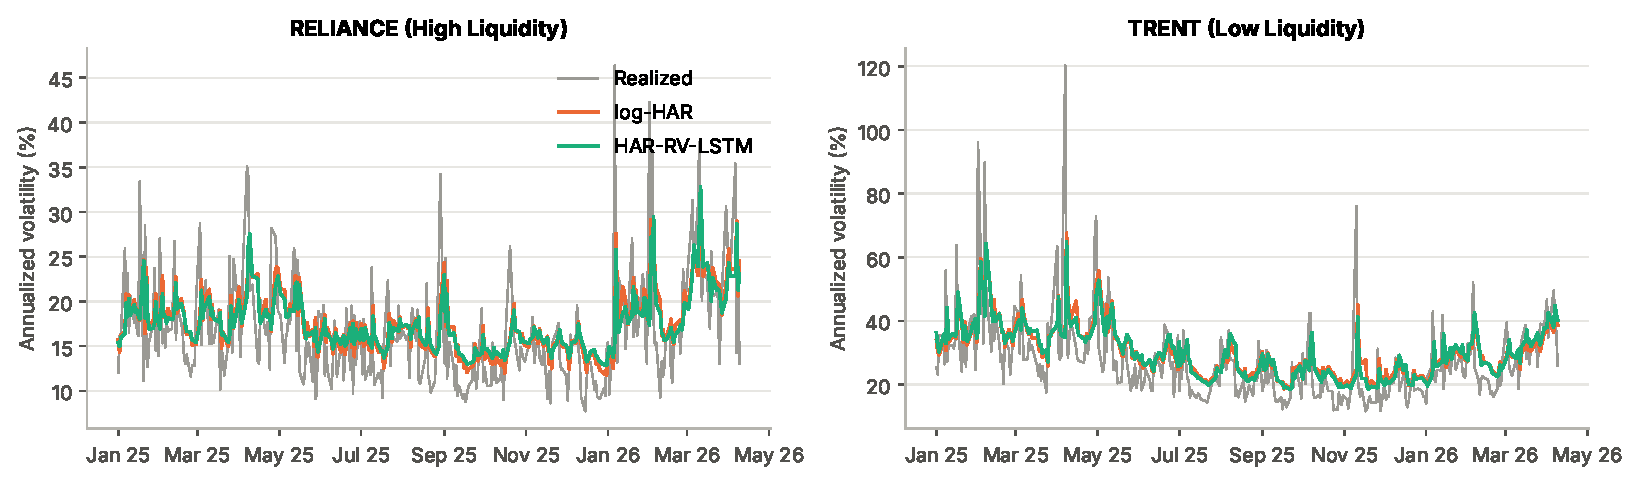
\includegraphics[width=\textwidth]{fig_example_stocks}
\caption{Realized and forecast volatility for a highly liquid (Reliance) and a less liquid (Trent) stock.}
\label{fig:examples}
\end{figure}

\section{What Changed from the First Version}
\label{sec:versions}

\begin{table}[htbp]
\centering
\caption{Test QLIKE in the first version of the project and after the corrections}
\label{tab:versions}
\small
\begin{adjustbox}{max width=\textwidth}
\begin{tabular}{lrrrr}
\toprule
Model & First version & Corrected & vs HAR-RV, first (\%) & vs HAR-RV, corrected (\%) \\
\midrule
HAR-RV & 0.4230 & 0.2286 & -- & -- \\
HAR-RV-LSTM & 0.3421 & 0.1935 & $-$19.1 & $-$15.4 \\
EGARCH-LSTM & 0.3950 & 0.2709 & $-$6.6 & +18.5 \\
log-HAR & -- & 0.1965 & -- & $-$14.0 \\
\bottomrule
\end{tabular}
\end{adjustbox}
\par\smallskip\parbox{0.95\textwidth}{\footnotesize\itshape First version: 29,830 stock-days, uncleaned RV with overnight gaps, EGARCH fitted on the full sample, liquidity groups from the mis-scaled slope (only 42\% of stocks keep the same group after the correction). The two columns are not on identical samples; compare the relative columns.}
\end{table}


A first version of the project reported a 19.1\% QLIKE gain for HAR-RV-LSTM and a 6.6\% gain for
EGARCH-LSTM over HAR-RV. A code review found three problems:
\begin{enumerate}
\item \textbf{Dirty RV.} RV included the overnight gap and bad prints (VBL on 14 June 2023 jumped from 322
to 644 and back within ten minutes). These spikes inflated level-HAR errors most. Cleaning cut HAR-RV's
test QLIKE from 0.423 to 0.229.
\item \textbf{Liquidity groups.} The slope-based measure divided signed volume by its own mean, which is
close to zero and differs across stocks, so the ranking was close to random (ICICI Bank ``Medium'',
Infosys ``Low''). Only 42\% of stocks keep their group under the corrected Amihud measure.
\item \textbf{EGARCH look-ahead.} EGARCH was estimated on 2016--2026, so its test-period features used
parameters fitted on test data. With training-only parameters, EGARCH-LSTM moves from 6.6\% better to
18.5\% worse than HAR-RV.
\end{enumerate}
The headline survives: HAR-RV-LSTM is still the best model. Its advantage is smaller and better
understood: most of it is the log transformation, and the true network gain is concentrated in less
liquid stocks.

\section{Where the Research Can Be Used}

\textbf{Options trading.} Almost all stocks in the sample have NSE stock options. A one-day RV forecast
is the realized-volatility leg of the volatility risk premium: comparing it with the option's implied
volatility indicates whether straddles or strangles are rich or cheap, and it sets the expected gamma
P\&L of a delta-hedged position. The liquidity result matters here: for illiquid names the LSTM's edge is
largest, and these are also the options where implied volatility is least efficient.

\textbf{Risk management and margins.} Next-day volatility drives Value-at-Risk, Expected Shortfall and
exposure limits. Brokers and clearing members can use stock-level forecasts to set margins and position
limits; a forecast 6\% above realized on average (LSTM) is safer than one 21\% above (HAR-RV), which ties up
capital, or one that under-reacts.

\textbf{Position sizing and volatility targeting.} Scaling positions by forecast volatility improves
risk-adjusted returns \citep{fleming2001,moreira2017}. Better forecasts on ordinary days, where this
model gains most, translate directly into steadier risk.

\textbf{Execution and market making.} Expected intraday volatility sets quoted spreads, inventory limits
and how fast to work an order. The gain is largest in less liquid stocks, where execution cost is highest.

\textbf{Surveillance.} The gap between realized and forecast RV flags unusual days (for example, the Adani
episode in February 2023) for exchanges, regulators and risk desks.

\textbf{Model choice in practice.} For the 30 or so most liquid stocks, log-HAR is as good as the LSTM and
far simpler. A pooled LSTM pays for itself across a broad, mixed-liquidity universe. Because the model
loses ground on spike days, it should be paired with a stress overlay rather than used alone in crises.

\section{Limitations and Further Work}

\begin{itemize}
\item \textbf{One test period}, mostly calm, with no ``turbulent'' days by training standards. Results in a
crisis may differ; re-training on a rolling window would test this.
\item \textbf{Survivorship}: the universe is today's NIFTY~100, so stocks that dropped out are missing.
\item \textbf{Intraday RV only}: the overnight gap is excluded from the target. A close-to-close
volatility forecast would need an overnight component.
\item \textbf{Inputs}: the LSTM sees only RV history. India VIX, jump and semivariance measures
\citep{bollerslev2016}, volume and market-wide RV are natural additions.
\item \textbf{Testing}: a Model Confidence Set \citep{hansen2011} and an economic test (option P\&L or VaR
back-test) would complete the evaluation.
\end{itemize}

\section{Conclusion}

Across 95 NSE stocks and 15 months of out-of-sample data, an LSTM fed with HAR inputs forecasts next-day
realized volatility best: 15\% better than HAR-RV and 1.6\% better than log-HAR, both significant. The
network's own gain is modest and concentrated in less liquid stocks and calm-to-normal markets. Models
built only on daily returns (EGARCH-LSTM) are clearly worse, and EGARCH information adds nothing once the
intraday history is known. Careful data cleaning and leak-free design changed the size of the results
more than the choice of model did.


\begin{thebibliography}{}

\bibitem[Amihud, 2002]{amihud2002}
Amihud, Y. (2002).
\newblock Illiquidity and stock returns: Cross-section and time-series effects.
\newblock {\em Journal of Financial Markets}, 5(1):31--56.

\bibitem[Andersen et~al., 2003]{andersen2003}
Andersen, T.~G., Bollerslev, T., Diebold, F.~X., and Labys, P. (2003).
\newblock Modeling and forecasting realized volatility.
\newblock {\em Econometrica}, 71(2):579--625.

\bibitem[Bollerslev et~al., 2016]{bollerslev2016}
Bollerslev, T., Patton, A.~J., and Quaedvlieg, R. (2016).
\newblock Exploiting the errors: A simple approach for improved volatility
  forecasting.
\newblock {\em Journal of Econometrics}, 192(1):1--18.

\bibitem[Bucci, 2020]{bucci2020}
Bucci, A. (2020).
\newblock Realized volatility forecasting with neural networks.
\newblock {\em Journal of Financial Econometrics}, 18(3):502--531.

\bibitem[Christensen et~al., 2023]{christensen2023}
Christensen, K., Siggaard, M., and Veliyev, B. (2023).
\newblock A machine learning approach to volatility forecasting.
\newblock {\em Journal of Financial Econometrics}, 21(5):1680--1727.

\bibitem[Corsi, 2009]{corsi2009}
Corsi, F. (2009).
\newblock A simple approximate long-memory model of realized volatility.
\newblock {\em Journal of Financial Econometrics}, 7(2):174--196.

\bibitem[Diebold and Mariano, 1995]{diebold1995}
Diebold, F.~X. and Mariano, R.~S. (1995).
\newblock Comparing predictive accuracy.
\newblock {\em Journal of Business \& Economic Statistics}, 13(3):253--263.

\bibitem[Fleming et~al., 2001]{fleming2001}
Fleming, J., Kirby, C., and Ostdiek, B. (2001).
\newblock The economic value of volatility timing.
\newblock {\em Journal of Finance}, 56(1):329--352.

\bibitem[Hansen et~al., 2011]{hansen2011}
Hansen, P.~R., Lunde, A., and Nason, J.~M. (2011).
\newblock The model confidence set.
\newblock {\em Econometrica}, 79(2):453--497.

\bibitem[Hochreiter and Schmidhuber, 1997]{hochreiter1997}
Hochreiter, S. and Schmidhuber, J. (1997).
\newblock Long short-term memory.
\newblock {\em Neural Computation}, 9(8):1735--1780.

\bibitem[Kim and Won, 2018]{kim2018}
Kim, H.~Y. and Won, C.~H. (2018).
\newblock Forecasting the volatility of stock price index: A hybrid model
  integrating {LSTM} with multiple {GARCH}-type models.
\newblock {\em Expert Systems with Applications}, 103:25--37.

\bibitem[Liu et~al., 2015]{liu2015}
Liu, L.~Y., Patton, A.~J., and Sheppard, K. (2015).
\newblock Does anything beat 5-minute {RV}? {A} comparison of realized measures
  across multiple asset classes.
\newblock {\em Journal of Econometrics}, 187(1):293--311.

\bibitem[Moreira and Muir, 2017]{moreira2017}
Moreira, A. and Muir, T. (2017).
\newblock Volatility-managed portfolios.
\newblock {\em Journal of Finance}, 72(4):1611--1644.

\bibitem[Nelson, 1991]{nelson1991}
Nelson, D.~B. (1991).
\newblock Conditional heteroskedasticity in asset returns: A new approach.
\newblock {\em Econometrica}, 59(2):347--370.

\bibitem[Newey and West, 1987]{neweywest1987}
Newey, W.~K. and West, K.~D. (1987).
\newblock A simple, positive semi-definite, heteroskedasticity and
  autocorrelation consistent covariance matrix.
\newblock {\em Econometrica}, 55(3):703--708.

\bibitem[Patton, 2011]{patton2011}
Patton, A.~J. (2011).
\newblock Volatility forecast comparison using imperfect volatility proxies.
\newblock {\em Journal of Econometrics}, 160(1):246--256.

\bibitem[Rahimikia and Poon, 2020]{rahimikia2020}
Rahimikia, E. and Poon, S.-H. (2020).
\newblock Machine learning for realised volatility forecasting.
\newblock SSRN Working Paper 3707796.

\bibitem[Zhang et~al., 2024]{zhang2024}
Zhang, C., Zhang, Y., Cucuringu, M., and Qian, Z. (2024).
\newblock Volatility forecasting with machine learning and intraday
  commonality.
\newblock {\em Journal of Financial Econometrics}, 22(2):492--530.

\end{thebibliography}


\clearpage
\appendix
\section*{Annex A. Additional Results}
\addcontentsline{toc}{section}{Annex A. Additional Results}
\floatplacement{table}{H}\floatplacement{figure}{H}

\begin{table}[H]
\centering
\caption{The ten highest-RV stock-days after cleaning}
\label{tab:topdays}
\small
\begin{adjustbox}{max width=\textwidth}
\begin{tabular}{llrrrl}
\toprule
Stock & Date & RV & Ann. vol (\%) & Return (\%) & Event \\
\midrule
ADANIENT & 2023-02-02 & 0.0855 & 464 & $-$33.1 & Adani sell-off after short-seller report \\
ADANIENT & 2023-02-03 & 0.0654 & 406 & $-$2.0 & Adani sell-off \\
ONGC & 2020-03-18 & 0.0645 & 403 & 3.6 & COVID-19 crash \\
KOTAKBANK & 2020-03-13 & 0.0629 & 398 & 0.7 & COVID-19: market-wide circuit, halt and rebound \\
BPCL & 2020-03-13 & 0.0624 & 396 & $-$0.1 & COVID-19: market-wide circuit, halt and rebound \\
ADANIPOWER & 2020-03-13 & 0.0500 & 355 & 4.9 & COVID-19: market-wide circuit, halt and rebound \\
BANKBARODA & 2020-03-13 & 0.0500 & 355 & 17.7 & COVID-19: market-wide circuit, halt and rebound \\
DRREDDY & 2019-02-15 & 0.0476 & 346 & $-$4.0 & stock-specific \\
CGPOWER & 2016-03-15 & 0.0441 & 333 & $-$17.9 & stock-specific \\
ADANIPORTS & 2023-02-02 & 0.0422 & 326 & $-$9.2 & Adani sell-off after short-seller report \\
\bottomrule
\end{tabular}
\end{adjustbox}
\end{table}

\begin{table}[H]
\centering
\caption{LSTM results across three random seeds}
\label{tab:seeds}
\small
\begin{adjustbox}{max width=\textwidth}
\begin{tabular}{lrrrrcr}
\toprule
Model & Valid mean & Valid s.d. & Test mean & Test s.d. & Test range & 3-seed average forecast \\
\midrule
HAR-RV-LSTM & 0.2264 & 0.0003 & 0.1940 & 0.0017 & 0.1926--0.1959 & 0.1935 \\
EGARCH-LSTM & 0.2709 & 0.0011 & 0.2713 & 0.0009 & 0.2703--0.2720 & 0.2709 \\
HAR-EGARCH-LSTM & 0.2189 & 0.0006 & 0.1935 & 0.0017 & 0.1916--0.1946 & 0.1931 \\
\bottomrule
\end{tabular}
\end{adjustbox}
\par\smallskip\parbox{0.95\textwidth}{\footnotesize\itshape QLIKE of each seed's network and of the forecast averaged over the three networks.}
\end{table}

\begin{table}[H]
\centering
\caption{Share of the 95 stocks on which a model has lower test QLIKE than the benchmark (\%)}
\label{tab:winrates}
\small
\begin{adjustbox}{max width=\textwidth}
\begin{tabular}{lrr}
\toprule
Model & Beats HAR-RV & Beats log-HAR \\
\midrule
log-HAR & 100 & -- \\
HAR-RV-LSTM & 100 & 70 \\
EGARCH-LSTM & 15 & 0 \\
\bottomrule
\end{tabular}
\end{adjustbox}
\end{table}

\begin{table}[H]
\centering
\caption{HAR coefficients, mean (s.d.) across stocks, estimated on 2016--2024}
\label{tab:harcoef}
\small
\begin{adjustbox}{max width=\textwidth}
\begin{tabular}{lrrrrr}
\toprule
Model & $\beta_0$ & $\beta_D$ & $\beta_W$ & $\beta_M$ & $\beta_D+\beta_W+\beta_M$ \\
\midrule
HAR-RV & 1.339 (0.924) & 0.229 (0.121) & 0.365 (0.171) & 0.125 (0.103) & 0.720 \\
log-HAR & $-$1.660 (0.422) & 0.347 (0.054) & 0.246 (0.058) & 0.212 (0.060) & 0.804 \\
\bottomrule
\end{tabular}
\end{adjustbox}
\par\smallskip\parbox{0.95\textwidth}{\footnotesize\itshape HAR-RV constant shown $\times10^{4}$.}
\end{table}

\begin{table}[H]
\centering
\caption{EGARCH(1,1)-t parameters across the 95 stocks (estimated on 2016--2022)}
\label{tab:egarch}
\small
\begin{adjustbox}{max width=\textwidth}
\begin{tabular}{lrrrr}
\toprule
Parameter & Mean & Median & 10th pct & 90th pct \\
\midrule
$\mu$ & 0.017 & 0.013 & $-$0.045 & 0.077 \\
$\omega$ & 0.146 & 0.070 & 0.035 & 0.266 \\
$\alpha$ & 0.198 & 0.164 & 0.097 & 0.328 \\
$\gamma$ & $-$0.042 & $-$0.044 & $-$0.091 & $-$0.004 \\
$\beta$ & 0.924 & 0.953 & 0.851 & 0.981 \\
$\nu$ & 4.783 & 4.703 & 3.740 & 5.747 \\
Share with $\gamma<0$ & \multicolumn{4}{l}{92\%} \\
\bottomrule
\end{tabular}
\end{adjustbox}
\end{table}


\begin{figure}[htbp]
\centering
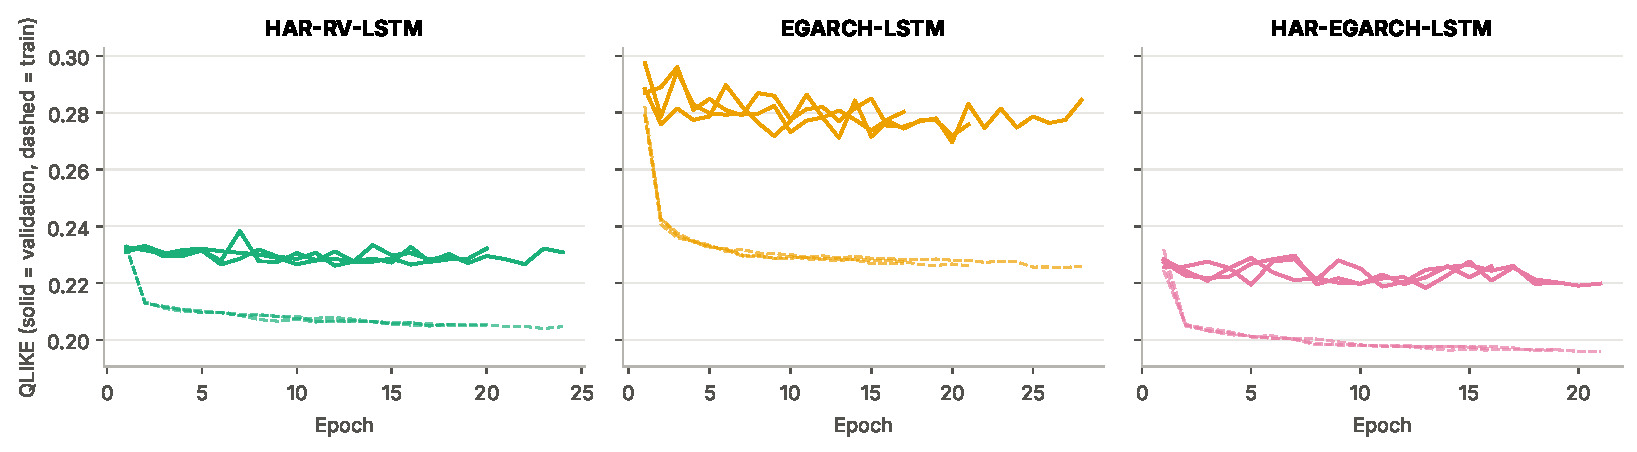
\includegraphics[width=\textwidth]{fig_training_curves}
\caption{Training (dashed) and validation (solid) QLIKE by epoch, three seeds per model.}
\label{fig:training}
\end{figure}

\begin{table}[H]
\centering
\caption{Test QLIKE for every stock, ordered by liquidity rank}
\label{tab:perstock}
\scriptsize
\begin{adjustbox}{max width=\textwidth}
\begin{tabular}{rlcrrr|rlcrrr}
\toprule
\# & Stock & L & log-HAR & LSTM & Gain\% & \# & Stock & L & log-HAR & LSTM & Gain\% \\
\midrule
1 & RELIANCE & H & 0.177 & 0.179 & $-$0.8 & 49 & DIVISLAB & M & 0.209 & 0.202 & +3.4 \\
2 & SBIN & H & 0.169 & 0.178 & $-$4.9 & 50 & GRASIM & M & 0.125 & 0.126 & $-$0.8 \\
3 & INFY & H & 0.159 & 0.159 & $-$0.1 & 51 & BEL & M & 0.221 & 0.215 & +2.5 \\
4 & ICICIBANK & H & 0.144 & 0.152 & $-$5.2 & 52 & AMBUJACEM & M & 0.167 & 0.161 & +3.3 \\
5 & MARUTI & H & 0.225 & 0.221 & +1.9 & 53 & GAIL & M & 0.175 & 0.174 & +0.4 \\
6 & TCS & H & 0.155 & 0.155 & +0.2 & 54 & RECLTD & M & 0.144 & 0.141 & +2.4 \\
7 & AXISBANK & H & 0.161 & 0.154 & +4.4 & 55 & BRITANNIA & M & 0.224 & 0.213 & +4.7 \\
8 & ITC & H & 0.325 & 0.314 & +3.3 & 56 & TVSMOTOR & M & 0.209 & 0.211 & $-$0.9 \\
9 & TMPV & H & 0.221 & 0.218 & +1.3 & 57 & HDFCAMC & M & 0.194 & 0.189 & +2.3 \\
10 & LT & H & 0.194 & 0.199 & $-$2.6 & 58 & PFC & M & 0.183 & 0.179 & +2.0 \\
11 & TATASTEEL & H & 0.172 & 0.172 & $-$0.3 & 59 & APOLLOHOSP & M & 0.240 & 0.235 & +1.9 \\
12 & HDFCBANK & H & 0.199 & 0.200 & $-$0.3 & 60 & GODREJCP & M & 0.235 & 0.233 & +1.0 \\
13 & SUNPHARMA & H & 0.200 & 0.199 & +0.3 & 61 & PIDILITIND & M & 0.157 & 0.155 & +0.9 \\
14 & HINDUNILVR & H & 0.267 & 0.267 & +0.0 & 62 & TATAPOWER & M & 0.187 & 0.187 & +0.0 \\
15 & KOTAKBANK & H & 0.146 & 0.146 & +0.0 & 63 & INDIGO & M & 0.233 & 0.230 & +1.3 \\
16 & ETERNAL & H & 0.265 & 0.256 & +3.5 & 64 & ZYDUSLIFE & L & 0.150 & 0.150 & +0.0 \\
17 & BHARTIARTL & H & 0.163 & 0.168 & $-$2.9 & 65 & TATACONSUM & L & 0.191 & 0.188 & +1.5 \\
18 & MM & H & 0.172 & 0.176 & $-$2.6 & 66 & BAJAJFINSV & L & 0.188 & 0.184 & +2.2 \\
19 & BAJFINANCE & H & 0.178 & 0.178 & $-$0.1 & 67 & ADANIENT & L & 0.191 & 0.187 & +2.4 \\
20 & ASIANPAINT & H & 0.298 & 0.296 & +0.5 & 68 & NESTLEIND & L & 0.194 & 0.188 & +3.2 \\
21 & HINDALCO & H & 0.173 & 0.169 & +1.9 & 69 & BOSCHLTD & L & 0.146 & 0.142 & +2.7 \\
22 & DRREDDY & H & 0.171 & 0.171 & +0.2 & 70 & EICHERMOT & L & 0.199 & 0.196 & +1.7 \\
23 & BPCL & H & 0.137 & 0.137 & $-$0.7 & 71 & SBILIFE & L & 0.242 & 0.234 & +3.5 \\
24 & ULTRACEMCO & H & 0.184 & 0.183 & +0.3 & 72 & SIEMENS & L & 0.217 & 0.214 & +1.8 \\
25 & TECHM & H & 0.160 & 0.159 & +0.8 & 73 & UNIONBANK & L & 0.184 & 0.180 & +2.0 \\
26 & ONGC & H & 0.192 & 0.196 & $-$2.1 & 74 & TORNTPHARM & L & 0.157 & 0.155 & +0.8 \\
27 & VEDL & H & 0.217 & 0.214 & +1.4 & 75 & SHREECEM & L & 0.138 & 0.141 & $-$2.7 \\
28 & COALINDIA & H & 0.156 & 0.156 & +0.0 & 76 & ADANIPOWER & L & 0.386 & 0.356 & +7.7 \\
29 & HCLTECH & H & 0.203 & 0.207 & $-$2.1 & 77 & HINDZINC & L & 0.177 & 0.173 & +2.0 \\
30 & JSWSTEEL & H & 0.217 & 0.216 & +0.5 & 78 & CUMMINSIND & L & 0.170 & 0.166 & +2.7 \\
31 & BANKBARODA & H & 0.160 & 0.159 & +0.8 & 79 & IRFC & L & 0.205 & 0.202 & +1.5 \\
32 & ADANIPORTS & H & 0.184 & 0.174 & +5.9 & 80 & LODHA & L & 0.212 & 0.172 & +19.2 \\
33 & CIPLA & M & 0.259 & 0.264 & $-$1.8 & 81 & LTM & L & 0.179 & 0.178 & +0.5 \\
34 & BAJAJ-AUTO & M & 0.178 & 0.180 & $-$0.9 & 82 & MAXHEALTH & L & 0.170 & 0.146 & +13.9 \\
35 & POWERGRID & M & 0.173 & 0.167 & +3.6 & 83 & MAZDOCK & L & 0.237 & 0.231 & +2.2 \\
36 & DLF & M & 0.155 & 0.153 & +1.8 & 84 & MUTHOOTFIN & L & 0.220 & 0.224 & $-$1.8 \\
37 & PNB & M & 0.204 & 0.190 & +6.6 & 85 & ABB & L & 0.230 & 0.231 & $-$0.6 \\
38 & TITAN & M & 0.214 & 0.205 & +4.2 & 86 & INDHOTEL & L & 0.164 & 0.172 & $-$4.9 \\
39 & WIPRO & M & 0.181 & 0.182 & $-$1.0 & 87 & BAJAJHLDNG & L & 0.208 & 0.213 & $-$2.1 \\
40 & JINDALSTEL & M & 0.151 & 0.154 & $-$2.0 & 88 & ADANIGREEN & L & 0.289 & 0.260 & +9.9 \\
41 & HDFCLIFE & M & 0.225 & 0.221 & +1.6 & 89 & HAL & L & 0.228 & 0.226 & +0.8 \\
42 & NTPC & M & 0.171 & 0.168 & +1.8 & 90 & CHOLAFIN & L & 0.199 & 0.192 & +3.3 \\
43 & DMART & M & 0.253 & 0.261 & $-$3.0 & 91 & VBL & L & 0.216 & 0.209 & +3.4 \\
44 & IOC & M & 0.157 & 0.154 & +2.2 & 92 & ADANIENSOL & L & 0.207 & 0.190 & +7.8 \\
45 & CANBK & M & 0.170 & 0.171 & $-$0.2 & 93 & TRENT & L & 0.229 & 0.230 & $-$0.4 \\
46 & SHRIRAMFIN & M & 0.203 & 0.197 & +3.3 & 94 & SOLARINDS & L & 0.189 & 0.190 & $-$0.0 \\
47 & MOTHERSON & M & 0.188 & 0.188 & +0.3 & 95 & CGPOWER & L & 0.250 & 0.247 & +1.1 \\
48 & UNITDSPR & M & 0.183 & 0.180 & +1.6 &  &  & & & &  \\
\bottomrule
\end{tabular}
\end{adjustbox}
\par\smallskip\parbox{0.95\textwidth}{\footnotesize\itshape L = liquidity group (H/M/L). LSTM = HAR-RV-LSTM. Gain = \% reduction in QLIKE against log-HAR.}
\end{table}


\clearpage
\section*{Annex B. Project Structure and Reproduction}
\addcontentsline{toc}{section}{Annex B. Project Structure and Reproduction}

\begin{tabularx}{\textwidth}{lX}
\toprule
Folder / file & Content \\
\midrule
\texttt{src/volforecast/} & All code: \texttt{config.py} (settings), \texttt{data\_pipeline.py}, \texttt{har.py},
\texttt{egarch.py}, \texttt{lstm.py}, \texttt{evaluation.py}, \texttt{plotting.py} \\
\texttt{notebooks/01--06} & Data cleaning and liquidity; HAR benchmarks; EGARCH features; HAR-RV-LSTM;
EGARCH-LSTM and ablation; model comparison \\
\texttt{data\_processed/} & Clean daily panel, EGARCH features, liquidity groups, universe \\
\texttt{results/} & Forecasts for every stock-day, all tables (CSV), trained network weights \\
\texttt{figures/} & All charts \\
\texttt{paper/} & This paper; \texttt{make\_tables.py} rebuilds every table from \texttt{results/tables} \\
\bottomrule
\end{tabularx}

Raw data (100 files, about 1 GB) are kept outside the project in \texttt{../data}. Running notebooks
01 to 06 in order reproduces every number in the paper.

\section*{Annex C. Code Excerpts}
\addcontentsline{toc}{section}{Annex C. Code Excerpts}

\textbf{Removing isolated spikes} (\texttt{data\_pipeline.py})
\begin{lstlisting}
def _remove_bad_ticks(log_close: pd.Series, day: pd.Series) -> pd.Series:
    """Blank out isolated price spikes that are reversed in the next bar.

    A spike is a 5-minute move larger than BAD_TICK_MIN_MOVE that the next bar undoes
    almost completely (e.g. VBL on 14-Jun-2023: 322 -> 644 -> 322). Genuine large moves
    (e.g. Adani stocks in Feb 2023) are not reversed and are kept.
    """
    lc = log_close.copy()
    for _ in range(3):  # repeat: removing one spike can reveal another
        prev = lc.groupby(day).ffill().groupby(day).shift(1)
        nxt = lc.groupby(day).bfill().groupby(day).shift(-1)
        r_in = lc - prev
        r_out = nxt - lc
        spike = (
            (r_in.abs() > C.BAD_TICK_MIN_MOVE)
            & (np.sign(r_in) != np.sign(r_out))
            & ((r_in + r_out).abs() < C.BAD_TICK_REVERSAL * r_in.abs())
        )
        if not spike.any():
            break
        lc[spike] = np.nan
    return lc
\end{lstlisting}

\textbf{Liquidity groups from training years only} (\texttt{data\_pipeline.py})
\begin{lstlisting}
def liquidity_groups(panel: pd.DataFrame, start=C.TRAIN_START, end=C.TRAIN_END) -> pd.DataFrame:
    """Rank stocks by 5-minute Amihud illiquidity measured in the TRAINING window only.

    ILLIQ = average over traded 5-minute bars of |return| / rupee volume  (Amihud, 2002).
    Lower ILLIQ = more liquid. Terciles: High / Medium / Low liquidity.
    Using training data only means the grouping contains no information from the
    validation or test years.
    """
    w = panel[(panel["Date"] >= start) & (panel["Date"] <= end)]
    agg = w.groupby("Symbol").agg(
        amihud_sum=("amihud_sum", "sum"), amihud_n=("amihud_n", "sum"),
        avg_daily_turnover_cr=("rupee_vol", lambda x: x.mean() / 1e7),
        train_days=("RV", "size"),
    )
    agg["ILLIQ"] = agg["amihud_sum"] / agg["amihud_n"] * 1e9   # per Rs 100 crore traded
    agg = agg.drop(columns=["amihud_sum", "amihud_n"]).sort_values("ILLIQ")
    agg["Liquidity_Rank"] = np.arange(1, len(agg) + 1)
    agg["Liquidity_Group"] = pd.qcut(
        agg["ILLIQ"], 3, labels=["High Liquidity", "Medium Liquidity", "Low Liquidity"]
    ).astype(str)
    return agg.reset_index()
\end{lstlisting}

\textbf{Splits assigned by target date} (\texttt{data\_pipeline.py})
\begin{lstlisting}
def split_by_target_date(p: pd.DataFrame):
    """Assign each row to a split by the date of its TARGET (t+1).

    This prevents the last training row from using a validation-day outcome.
    """
    d = p["Date_t1"]
    train = p[(d >= C.TRAIN_START) & (d <= C.TRAIN_END)].copy()
    valid = p[(d >= C.VALID_START) & (d <= C.VALID_END)].copy()
    test = p[(d >= C.TEST_START) & (d <= C.TEST_END)].copy()
    return train, valid, test
\end{lstlisting}

\textbf{HAR and log-HAR regression} (\texttt{har.py})
\begin{lstlisting}
def _fit_predict(train: pd.DataFrame, apply: pd.DataFrame, log: bool):
    X = train[HAR_FEATURES].to_numpy()
    y = train[TARGET].to_numpy()
    Xa = apply[HAR_FEATURES].to_numpy()
    if log:
        X, y, Xa = np.log(X), np.log(y), np.log(Xa)
    fit = sm.OLS(y, sm.add_constant(X, has_constant="add")).fit()
    pred = fit.predict(sm.add_constant(Xa, has_constant="add"))
    if log:
        pred = np.exp(pred + fit.mse_resid / 2)
    params = dict(zip(["const", "beta_D", "beta_W", "beta_M"], fit.params))
    return pred, params
\end{lstlisting}

\textbf{EGARCH without look-ahead} (\texttt{egarch.py})
\begin{lstlisting}
def egarch_features(panel: pd.DataFrame, symbols, fit_end: str = C.TRAIN_END):
    feats, params = [], []
    for sym in symbols:
        s = panel[panel["Symbol"] == sym].sort_values("Date")
        r = s.set_index("Date")["ret_cc"].astype(float)
        r_fit = r[r.index <= fit_end]
        with warnings.catch_warnings():
            warnings.simplefilter("ignore")
            res = arch_model(r_fit, mean="Constant", vol="EGARCH", p=1, o=1, q=1,
                             dist="t").fit(disp="off", show_warning=False)
            fixed = arch_model(r, mean="Constant", vol="EGARCH", p=1, o=1, q=1,
                               dist="t").fix(res.params)
        feats.append(pd.DataFrame({
            "Symbol": sym, "Date": r.index,
            "EGARCH_Vol": fixed.conditional_volatility.to_numpy(),
            "EGARCH_Resid": fixed.std_resid.to_numpy(),
        }))
        params.append({"Symbol": sym, **res.params.to_dict(), "n_fit": len(r_fit),
                       "converged": res.convergence_flag == 0})
    return pd.concat(feats, ignore_index=True), pd.DataFrame(params)
\end{lstlisting}

\textbf{Network and loss} (\texttt{lstm.py})
\begin{lstlisting}
class VolatilityLSTM(nn.Module):
    """2-layer LSTM (64 units) + stock embedding (8) + dense head (64-32-1).

    The output is exp(z + c), where c is the average log RV of the training targets.
    The exponential keeps every forecast positive, which QLIKE requires.
    """

    def __init__(self, n_features: int, n_stocks: int, log_rv_mean: float,
                 hidden: int = 64, layers: int = 2, emb_dim: int = 8, dropout: float = 0.2):
        super().__init__()
        self.embedding = nn.Embedding(n_stocks, emb_dim)
        self.lstm = nn.LSTM(n_features, hidden, num_layers=layers, batch_first=True,
                            dropout=dropout)
        self.head = nn.Sequential(
            nn.Dropout(dropout),
            nn.Linear(hidden + emb_dim, 64), nn.ReLU(),
            nn.Linear(64, 32), nn.ReLU(),
            nn.Linear(32, 1),
        )
        self.register_buffer("c", torch.tensor(float(log_rv_mean)))

    def forward(self, x, stock_id):
        _, (h, _) = self.lstm(x)
        z = self.head(torch.cat([h[-1], self.embedding(stock_id)], dim=1)).squeeze(-1)
        return torch.exp(z.clamp(-15, 15) + self.c)
\end{lstlisting}
\begin{lstlisting}
class QLIKELoss(nn.Module):
    """QLIKE = RV/h - log(RV/h) - 1 (Patton, 2011). Zero only when h = RV."""

    def forward(self, h, rv):
        ratio = rv / h
        return (ratio - torch.log(ratio) - 1).mean()
\end{lstlisting}

\textbf{Training with early stopping} (\texttt{lstm.py})
\begin{lstlisting}
def train_one_seed(X, meta, train_idx, valid_idx, n_stocks, seed, verbose=True):
    """Train with early stopping on validation QLIKE; return model and history."""
    torch.manual_seed(seed)
    np.random.seed(seed)
    c = float(np.log(meta[C.TARGET].to_numpy()[train_idx]).mean())
    model = VolatilityLSTM(X.shape[2], n_stocks, c)
    opt = torch.optim.Adam(model.parameters(), lr=C.LEARNING_RATE, weight_decay=C.WEIGHT_DECAY)
    sched = torch.optim.lr_scheduler.ReduceLROnPlateau(opt, factor=0.5, patience=3, min_lr=1e-6)
    loss_fn = QLIKELoss()
    train_dl = _loader(X, meta, train_idx, True)
    valid_dl = _loader(X, meta, valid_idx, False)

    best, best_state, wait, hist = np.inf, None, 0, []
    for epoch in range(1, C.MAX_EPOCHS + 1):
        model.train()
        tr = 0.0
        for xb, yb, sb in train_dl:
            opt.zero_grad()
            loss = loss_fn(model(xb, sb), yb)
            loss.backward()
            nn.utils.clip_grad_norm_(model.parameters(), 1.0)
            opt.step()
            tr += loss.item() * len(yb)
        tr /= len(train_idx)
        model.eval()
        with torch.no_grad():
            va = sum(loss_fn(model(xb, sb), yb).item() * len(yb) for xb, yb, sb in valid_dl)
        va /= len(valid_idx)
        sched.step(va)
        hist.append({"Seed": seed, "Epoch": epoch, "Train_QLIKE": tr, "Validation_QLIKE": va,
                     "Learning_Rate": opt.param_groups[0]["lr"]})
        if verbose:
            print(f"seed {seed} | epoch {epoch:2d} | train {tr:.4f} | valid {va:.4f}", flush=True)
        if va < best - 1e-5:
            best, best_state, wait = va, copy.deepcopy(model.state_dict()), 0
        else:
            wait += 1
            if wait >= C.PATIENCE:
                break
    model.load_state_dict(best_state)
    return model, pd.DataFrame(hist)
\end{lstlisting}

\textbf{Panel Diebold--Mariano test} (\texttt{evaluation.py})
\begin{lstlisting}
def dm_test(df, a, b, metric="QLIKE", lags=5, target=TARGET):
    """Panel Diebold-Mariano test.

    Loss differences are averaged across stocks for each day, then the mean of that
    daily series is tested with Newey-West (HAC) standard errors. A positive mean
    difference means model b has the lower loss.
    """
    s = _daily_loss_diff(df, a, b, metric, target)
    fit = sm.OLS(s.to_numpy(), np.ones(len(s))).fit(cov_type="HAC", cov_kwds={"maxlags": lags})
    return {"Metric": metric, "Model A": a, "Model B": b, "Mean diff (A-B)": s.mean(),
            "t-stat": fit.tvalues[0], "p-value": fit.pvalues[0], "Days": len(s)}
\end{lstlisting}

\end{document}
